\hspace{-1.4mm}[13~r\textsuperscript{o}] angulum rectum, et eadem facilitate intelligetur, quomodo ope Tubi \edtext{evertentis}{\lemma{}\Bfootnote{evertentis \textit{erg. L}}} inversi (\textit{Reverse-Tube}\edtext{}{\lemma{\textit{Reverse-Tube}}\Cfootnote{a.a.O., S. 58.}}) quilibet angulus intra quadrantem\protect\index{Sachverzeichnis}{quadrans} et duos angulos rectos possit sumi. Quod ut sit lectori paulo planius sit \textit{ccccc} in duodecima figura inferior Tubus, aut fixa dioptra\protect\index{Sachverzeichnis}{dioptra}, \textit{s} cavitas aut cellula-oculi (\textit{Eye-cell}\edtext{}{\lemma{\textit{Eye-cell}}\Cfootnote{a.a.O., S. 58.}}), \textit{tr} rotundum frustum (\textit{round piece}\edtext{}{\lemma{\textit{round piece}}\Cfootnote{a.a.O., S. 58.}}) ferens reflexivum Metallum \textit{gg}. Quod effectum est in gyrum circumagit et ita reflexivum Metallum \textit{gg} fixum ad ipsum in Tubo simul circumagitur cum ipso. \textit{siklmx} repraesentet radium \textit{passing forwards by the Eye-glass, Thread-sight and Object-glass;}\edtext{}{\lemma{\textit{Object-glass;}}\Cfootnote{a.a.O., S. 58.}} \edtext{inde rotundo hoc frusto}{\lemma{inde}\Bfootnote{\textit{(1)} rotundum haec frustum \textit{(2)} rotundo hoc frusto \textit{L}}} \textit{tr} circumacto et facto \textit{rt}, ut repraesentatum est in 13 figura, et cum ipso Metallo reflexivo \textit{gg} hic per \textit{qq} notato, eodem modo circumacto. Linea \textit{sqklmy} repraesentabit radium reflexum, et retrorsum \edtext{venientem per}{\lemma{venientem}\Bfootnote{\textit{(1)} ope \textit{(2)} per \textit{L}}} reflexivum Metallum \textit{qq} oculare\protect\index{Sachverzeichnis}{ocular} vitrum \textit{k} dioptricum filum \textit{l}, et vitrum objectivum \textit{y}. Mensura anguli invenietur eodem apparatu nempe cochleae quantum enim monstraret antea angulum minorem esse quadrante\protect\index{Sachverzeichnis}{quadrans}, tanto nunc monstrat majorem inversa parte adhibita. Superest tantum ostendendum; \textso{primo} quomodo hae duae Dioptrae\protect\index{Sachverzeichnis}{dioptra} Telescopicae\protect\index{Sachverzeichnis}{telescopium} locatae in Tubo, possint exacte servire ad videndum prorsum et retrorsum in eadem linea recta. Et \textso{secundo} quomodo accommodari possit ad Telescopium\protect\index{Sachverzeichnis}{telescopium} fixatum super mobili brachio quadrantis\protect\index{Sachverzeichnis}{quadrans}, ita ut agnosci possit \textit{when the} \textit{Divisions-Angle} \edtext{\textit{begins,}}{\lemma{\textit{begins},}\Cfootnote{a.a.O., S. 59.}} et quando aperiuntur ad quadrantem\protect\index{Sachverzeichnis}{quadrans}, angulum rectum, vel 90 graduum. Nonnisi ista ad tantam certitudinem habeantur quantae capax est divisio coch\-learis, et distinctio
\pend
\vspace{1.2em}
\count\Afootins=1200
\count\Bfootins=1200
\count\Cfootins=1200
\begin{center}                    
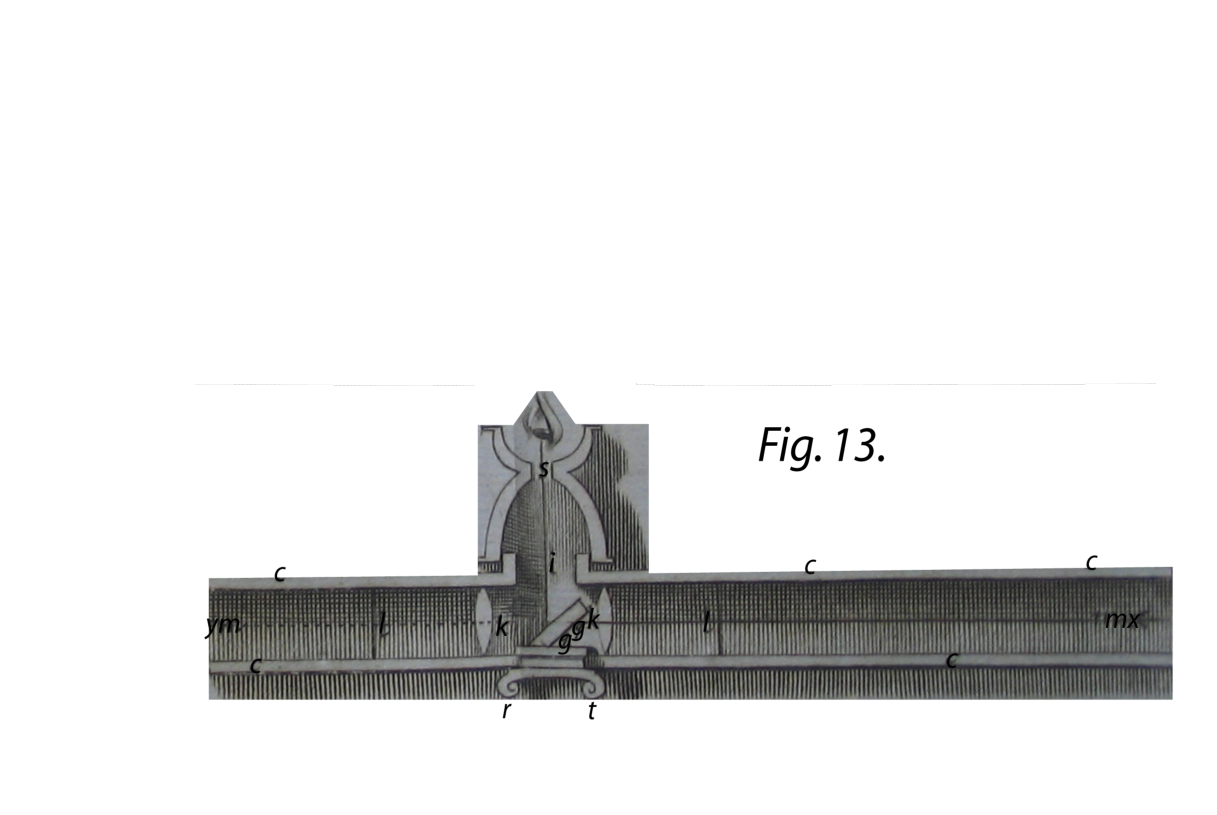
\includegraphics[trim = 0mm 0mm 0mm 1mm, clip, width=1\textwidth, angle=-0.5]{images/LH0351506_013r-dext13.pdf}\newline
\centering
[\textit{Fig. 4; erg. Hrsg. nach Hooke Fig. 13}]
\end{center}
\pstart\noindent Telescopica\protect\index{Sachverzeichnis}{telescopium}, et nisi perpendicularitas certa sit, omnis alius labor erit inutilis. \textso{Quoad primum} ut \edtext{fixentur fila dioptrica}{\lemma{fixentur}\Bfootnote{\textit{(1)} Dioptrae\protect\index{Sachverzeichnis}{dioptra} \textit{(2)} fila dioptrica \textit{L}}} utriusque Telescopii\protect\index{Sachverzeichnis}{telescopium} in eodem tubo, ita ut directe introrsum et retrorsum respiciant; cura adhibenda est, ut unum quodque ex quatuor vitris, hoc est duo vitra objectiva et duo ocularia\protect\index{Sachverzeichnis}{ocular}, ita firme et secure fixari possint in Tubo, ut nequeant \edtext{ulla vi}{\lemma{ulla}\Bfootnote{\textit{(1)} arte \textit{(2)} vi \textit{L}}} removeri ac disturbari. Sed hoc ita facile esse puto, ut non sit opus describere viam id praestandi. Secundo cura adhibenda, ne Tubi incurventur. Tertio unum ex filis dioptricis fixum esse debet ita ut vitra, et ita ut intersectio filorum ad crucem sit quoad ejus fieri potest in axe vitri objectivi et ocularis\protect\index{Sachverzeichnis}{ocular}; alterum filum dioptricum relinqui debet liberum donec multis experientiis inveniatur exacte in eadem linea cum priore, cujus rei praestandae modum nunc describam. Sint duo fila se ad angulos rectos secantia, unum perpendiculare alterum horizontale. Cura adhibenda, ut ambo jaceant exacte in eadem linea cum horizontali et perpendiculari \edtext{filis aliarum}{\lemma{}\Bfootnote{filis \textbar\ aliarum \textit{streicht Hrsg.} \textbar\ aliarum \textit{L}}} dioptrarum\protect\index{Sachverzeichnis}{dioptra}: et cum in finem sint \textit{two frames of brass,}\edtext{}{\lemma{\textit{brass},}\Cfootnote{a.a.O., S. 59.}} crassitie cavitatis Tubi habere ea opus est \edtext{\textit{groves}}{\lemma{\textit{groves}}\Cfootnote{a.a.O., S. 59.}} (gruben fossas) recipiendis ipsis aptas, in quibus ope cochlearum possint moveri \edtext{\textit{to and fro,}}{\lemma{\textit{to and fro},}\Cfootnote{a.a.O., S. 59.}} ut accommodentur. Postea opus est jungere ita exacte ut fila se tangere possint. Tertio opus est ut se exacte intersecent in foco vitrorum objectivi et ocularis\protect\index{Sachverzeichnis}{ocular}. \edtext{\textit{One of those frames}}{\lemma{\textit{frames}}\Cfootnote{a.a.O., S. 59.}} ducet filum perpendiculare, et ope cochleae in latere tubi mobile erit in latus dextrum aut sinistrum prout opus erit. \textit{The other frame}\edtext{}{\lemma{\textit{frame}}\Cfootnote{a.a.O., S. 59f.}} ducet filum horizontale, et ope cochleae in fastigio Tubi, fiet ita ut possit cadere et ascendere in Tubo, prout opus. His factis ex summitate turris vel alterius stationis \edtext{unde}{\lemma{}\Bfootnote{unde \textit{erg. L}}} duo opposita loca in distantia notabili v. g. \rule[-4mm]{0mm}{10mm}$\displaystyle\frac{1}{2}$ \edtext{\textit{mile, or a mile or two}}{\lemma{\textit{mile},}\Bfootnote{\textit{(1)} \textit{item one} \textit{(2)} \textit{or a mile or two} \textit{L}}}\edtext{}{\lemma{\textit{two},}\Cfootnote{a.a.O., S. 60.}} facile videri possint, inveni duo puncta quae primo inspectu per tua vitra invenis monstrari intersectione filorum dioptricorum, nota ea diligenter, ut certus sis red-inveniri \edtext{posse amotis vitris; quo facto circumage extremitates tubi}{\lemma{posse}\Bfootnote{\textit{(1)} \textbar\ amotis vitris \textit{erg.} \textbar\ quo facto circumage \textit{(2)} amotis \textit{(a)} Tubis \textit{(b)} vitris; quo facto circumage extremitates tubi \textit{L}}}, et (si ponas te introspexisse ab ortu versus occasum) inverte et partem orientalem fac esse occidentalem et contra, et inveni et duo eadem puncta rursus, inde dirigens partem quae habet fila fixa ad punctum ante visum dioptris mobilibus, quod certus es videre \textit{within the compas of your Eye-glass}\edtext{}{\lemma{\textit{Eye-glass}}\Cfootnote{a.a.O., S. 60.}} et observa quantum fila se secantia inde remota sint, versus
\pend
\newpage
\pstart 
%\begin{wrapfigure}{l}{0.5\textwidth}                    
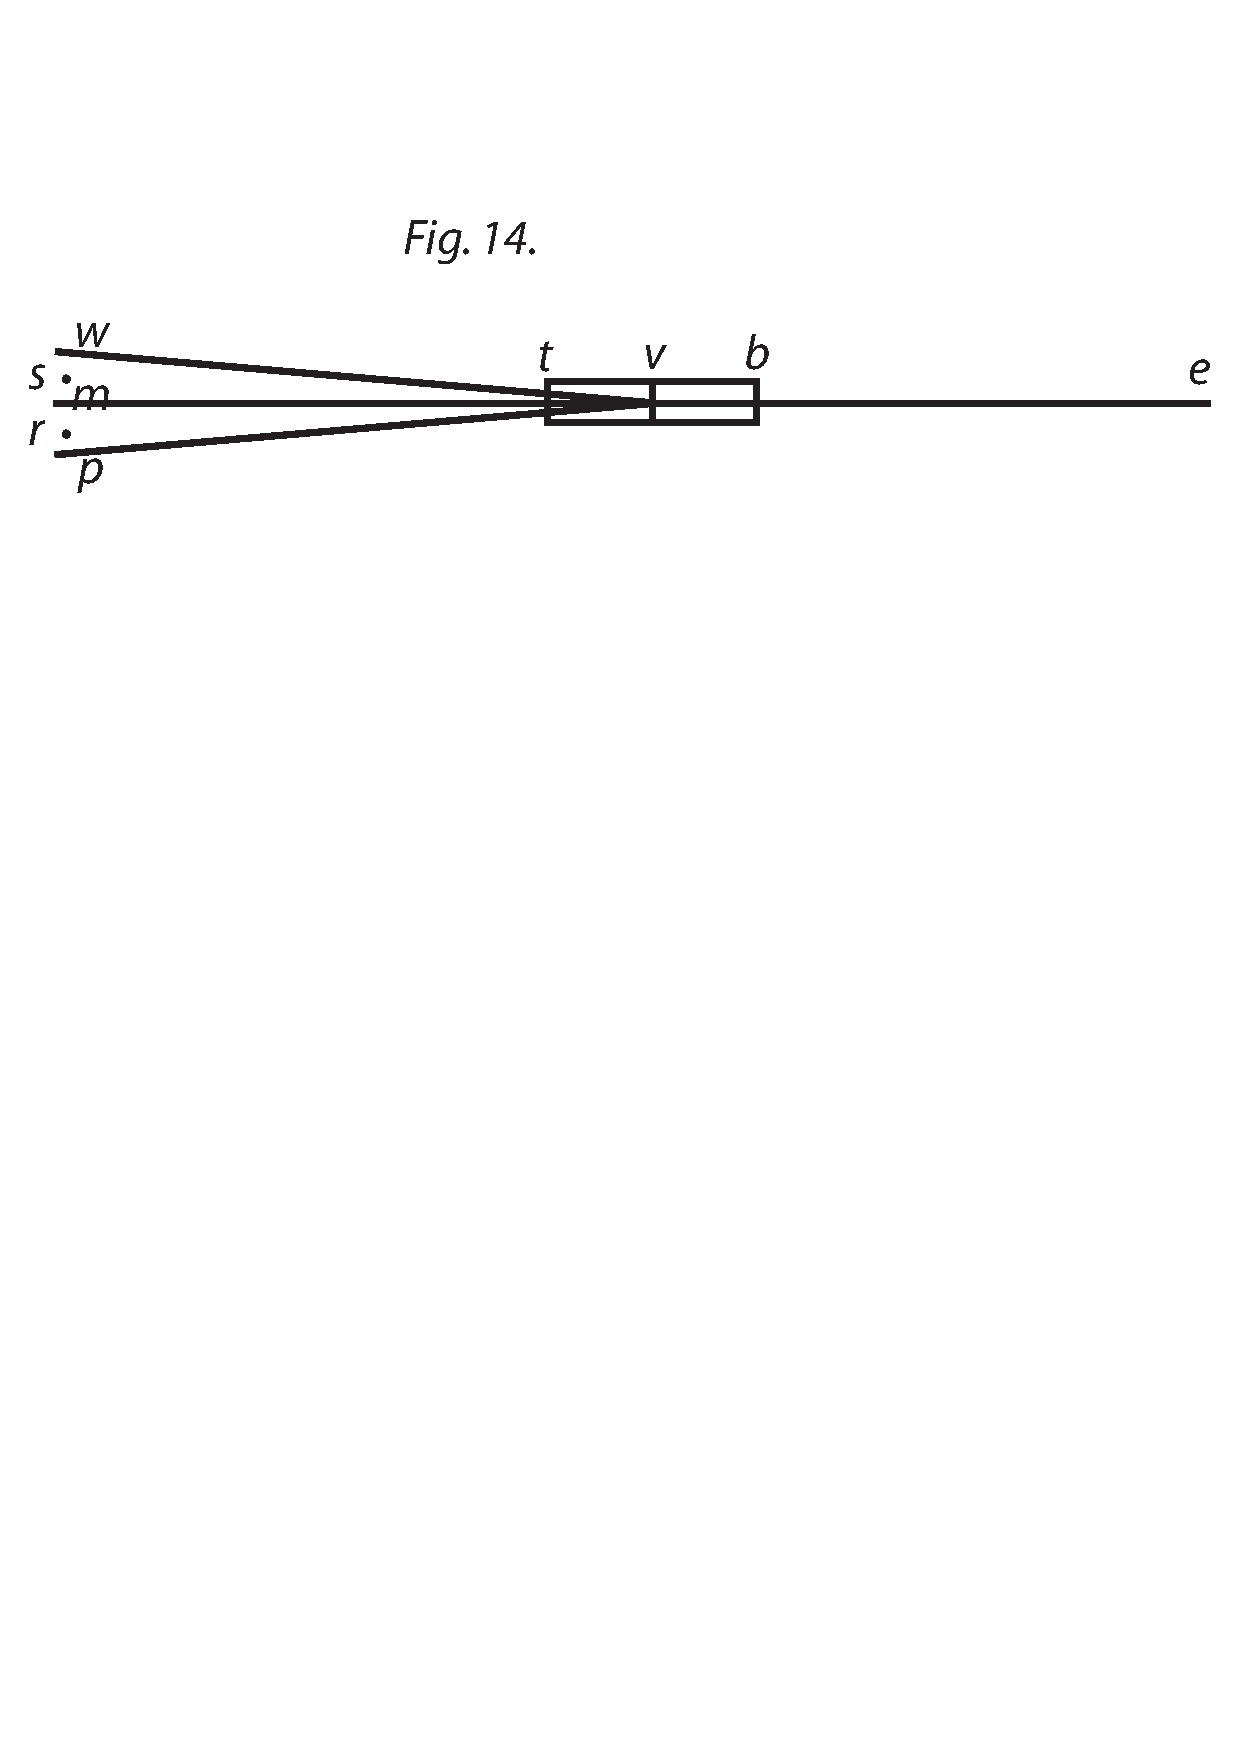
\includegraphics[trim = 0mm -5mm 0mm 0mm, clip,width=0.7\textwidth]{images/LH0351506_013r-dext14.pdf}\\
\centering \rule[0pt]{0mm}{0pt}[\textit{Fig. 5; erg. Hrsg. nach Hooke Fig. 14}]
%\end{wrapfigure}
\pend
\vspace{1em}
\pstart
\noindent \setline{1}Austrum vel Septentrionem sursum vel deorsum, inde quam prope potes, aestimatione hanc differentiam biseca et ope cochlearum \edtext{\textit{move the frames,}}{\lemma{\textit{move the frames,}}\Cfootnote{a.a.O., S. 60.}} ita ut fila sint in medio inter duo puncta: inde \edtext{rursus nota ea}{\lemma{rursus}\Bfootnote{\textit{(1)} observa ea \textit{(2)} nota ea \textit{L}}} puncta filis monstrata,
%\begin{wrapfigure}{l}{0.5\textwidth}                    
%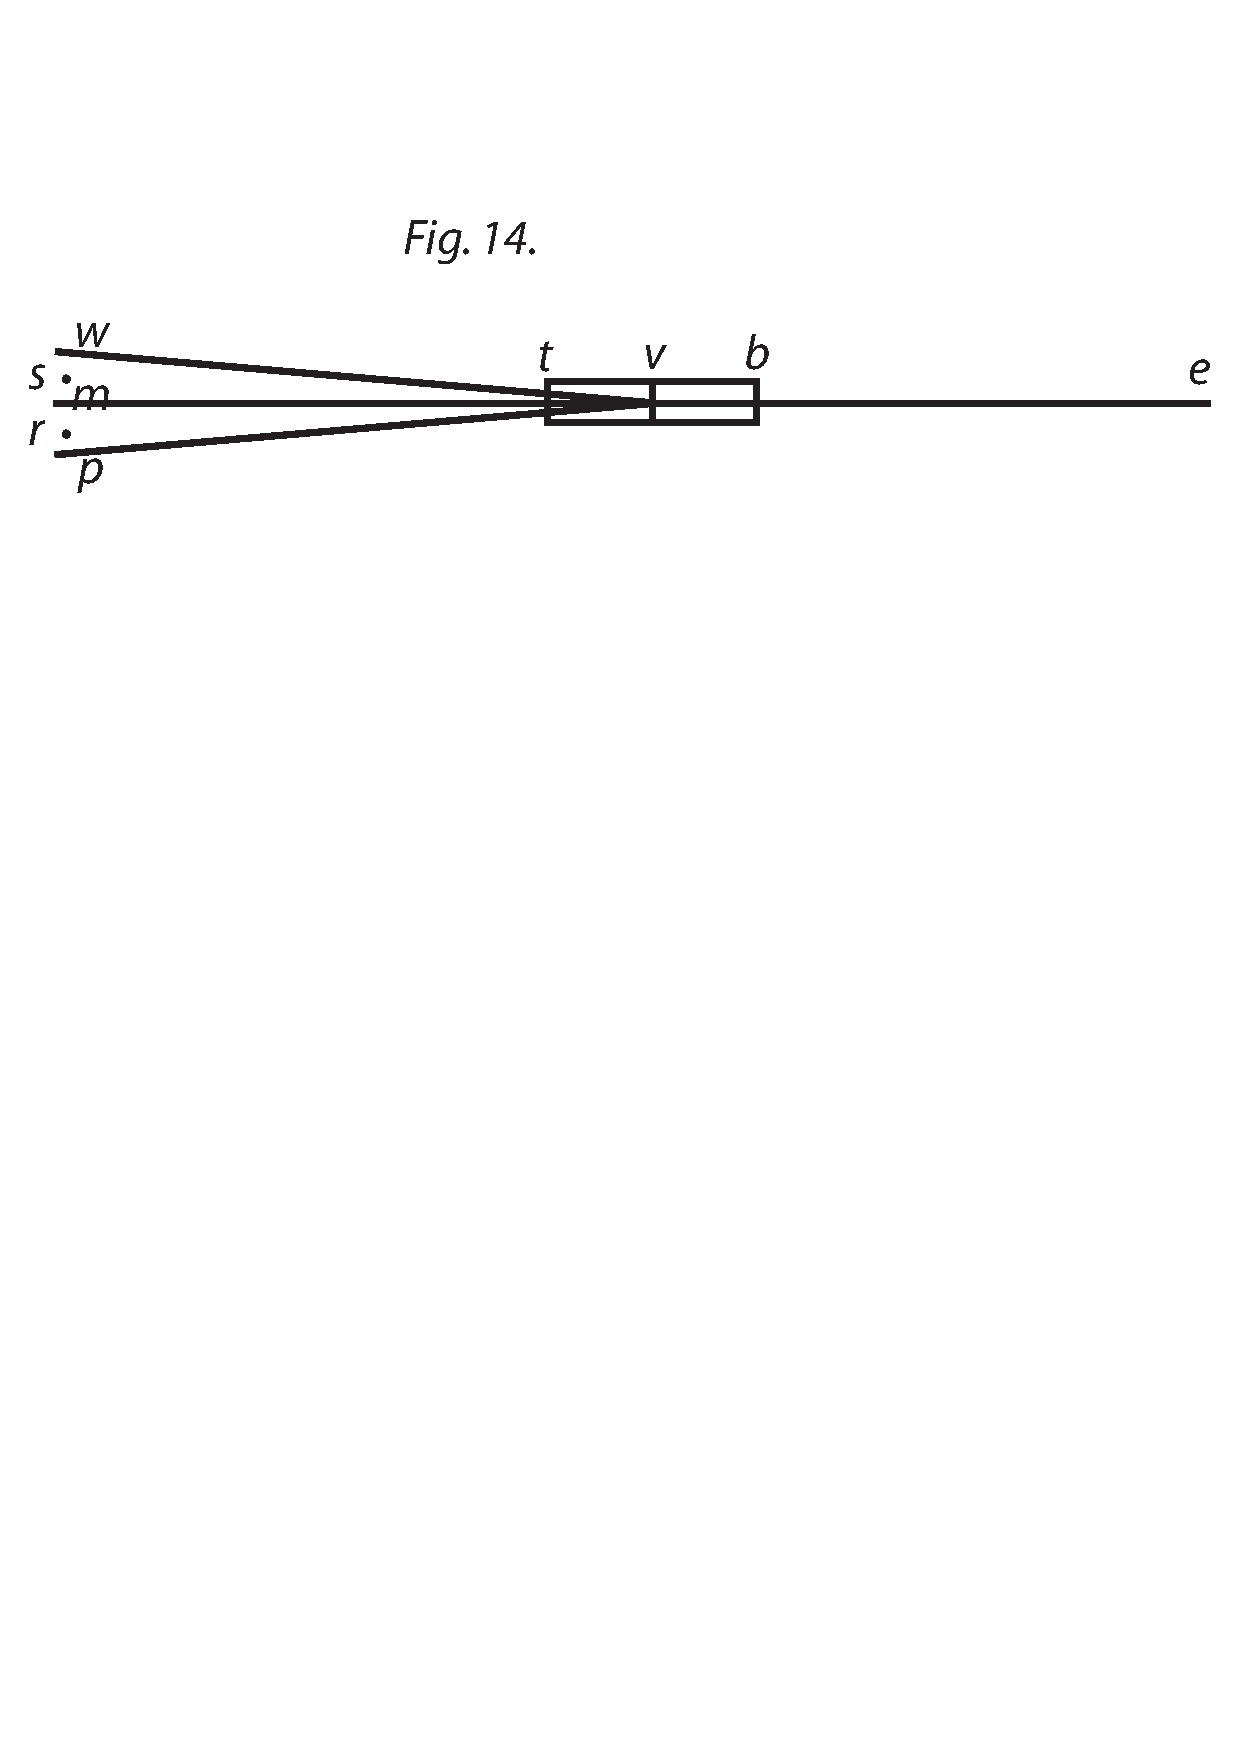
\includegraphics[width=0.5\textwidth]{images/LH0351506_013r-dext14.pdf}\\
%\rule[0pt]{3mm}{0pt}[\textit{Fig. 5; erg. Hrsg. nach Hooke Fig. 14}]
%\end{wrapfigure}
et [(]\textit{turn}\edtext{}{\lemma{\textit{turn}}\Cfootnote{a.a.O., S. 60.}}[)] circumage Tubum; hoc fac toties, donec circumacto tubo videas eadem puncta intersectionibus filorum notata, per quodcunque extremum introspicias, et hoc facto tubus erit exactus ad usum. Ratio hujus accommodationis plana illi qui inspexerit figuram 14. Pone enim \textit{v} repraesentare medium Tubi \textit{tvb} vel locum oculi, et \textit{w} repraesentare objectum visum occidentaliter, et \textit{e} objectum orientale, primo visu, inde servato exacte Tubi medio in eodem puncto \textit{u}, et circumagendo extremum Tubi \textit{t} versus orientem, et extremum \textit{b} versus occidentem et inveni primo objectum orientale \textit{e}; et inveniendo intersectionem nunc dirigere ad punctum \textit{p}, et non ad punctum \textit{w}. Divide distantiam inter puncta \textit{w} et \textit{p}, quam potes exacte in duas partes quod 